%% University of Tübingen Academic Poster Template
% Required Compiler: LuaLaTeX

\documentclass[final]{beamer}


% ====================
% Packages
% ====================

\usepackage[T1]{fontenc}
\usepackage{lmodern}
\usepackage{tcolorbox}
% \usepackage[size=custom,width=120,height=72,scale=1.0]{beamerposter} % default
\usepackage[orientation=landscape,size=a0,scale=1.4]{beamerposter} % custom
% scale: scaling factor of all font

\usetheme{gemini}
\usecolortheme{Tuebingen} % Customize in beamercolorthemeTuebingen.sty

\usepackage{graphicx}
\usepackage{booktabs}
\usepackage{tikz}
\usepackage{pgfplots}
\pgfplotsset{compat=1.14}
\usepackage{anyfontsize}

% ====================
% Lengths
% ====================

% If you have N columns, choose \sepwidth and \colwidth such that
% (N+1)*\sepwidth + N*\colwidth = \paperwidth
\newlength{\sepwidth}
\newlength{\colwidth}
\setlength{\sepwidth}{0.025\paperwidth}
\setlength{\colwidth}{0.3\paperwidth}

\newcommand{\separatorcolumn}{\begin{column}{\sepwidth}\end{column}}

% ====================
% Title
% ====================

\title{Behaviour of Pupil Diameter in Authoritative Control Interventions in Driving Automation}

\author{Lalitha Sivakumar \inst{1} \and Liza Dixon \inst{2}}

\institute[shortinst]{\inst{1} University of Tübingen \samelineand \inst{2} Robert Bosch GmbH}

% ====================
% Footer (optional)
% ====================

\footercontent{
  \href{https://tinyurl.com/wip2825-autoui24}{https://tinyurl.com/wip2825-autoui24} \hfill
  AutomativeUI Conference, Stanford, CA, USA, September 2024 \hfill
  \href{mailto: lalitha.sivakumar@student.uni-tuebingen.de}{ lalitha.sivakumar@student.uni-tuebingen.de}}
% (can be left out to remove footer)

% ====================
% Logo (optional)
% ====================

% use this to include logos on the left and/or right side of the header:
\logoleft{
\includegraphics[height=4cm]{images/logo_uni_white.pdf}}
\logoright{
\includegraphics[height=3cm]{images/Bosch-Logo.png}}

% ====================
% Body
% ====================

\begin{document}

\begin{frame}[t]
\begin{columns}[t]
\separatorcolumn

\begin{column}{\colwidth}

\begin{block}{The Experiment}

    A driving simulation study with \textbf{authoritative control interventions}, where the ADS initiates a control transition leading to a total loss of driver authority. They are of two types:
    \begin{itemize}
        \item Type 1 $T_1$, \textbf{Blocking} -- driver is blocked from taking control
        \item Type 2 $T_2$, \textbf{Takeaway} -- automation takes control away from the driver
    \end{itemize}
    
    \emph{N} = 18 drivers experienced 4 scenarios in 2 HMI designs:
 
    \begin{figure}
      \centering
      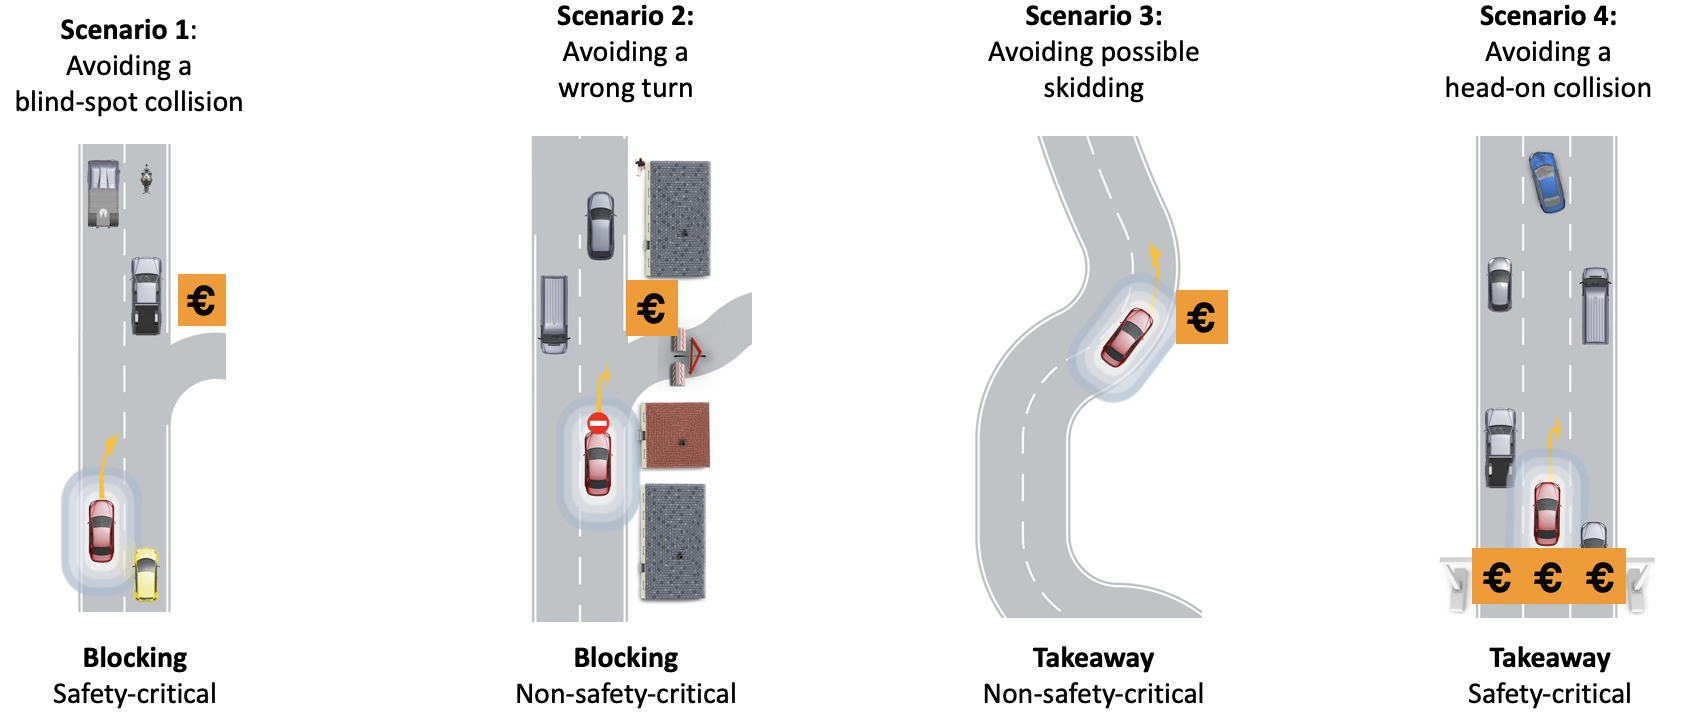
\includegraphics[width=0.90\linewidth]{scenarios.png}
      \caption{Overview of scenarios and intervention types (144 trials).}
      \label{fig:enter-label}
    \end{figure}

    \begin{alertblock}{Research Questions}
     {Can driver \textit{physiological arousal} be detected through changes in pupil dilation during an authoritative control intervention?
     \begin{itemize}
         \item Q1. Do these interventions affect pupil diameter?
         \item Q2. Does the intervention type or scenario criticality affect pupil diameter?
         \item Q3. What is the relationship between pupil dilation and variables like driver \texttt{age}, \texttt{valence} and their prior experience with automation (\texttt{autexp})?
     \end{itemize}
     
     }
    \end{alertblock}

\end{block}

    % \begin{*figure}
    % \hspace*{-\oddsidemargin}
    % \begin{flushedleft}
    %     \centering
    %     
\includegraphics[width=0.2\linewidth]{qrcode.png}
    %     \label{qrcode1}
    % \end{flushedleft}
    % \end{*figure}

  \begin{block}{Dilation between intervention phases -- \texttt{pdelt}}

    \begin{equation}
        \textcolor{utred}{\Delta PD\%} = \frac{{PD}_{\text{during}} - {PD}_{\text{before}}}{{PD}_{\text{before}}} \times 100
    \end{equation}

    
    \vspace{2cm}
    \end{block}
\end{column}

\separatorcolumn

\begin{column}{\colwidth}

\begin{block}{Q1. Minimal Baseline-Adjusted Dilation}
The baseline pupil diameter is calculated as the average of \( k \) points prior to the \( T_1 \) or \( T_2 \) intervention:
\begin{equation}
PD_{\text{baseline}} = \frac{1}{k} \sum_{i=1}^{k} PD_{\text{before}}
\end{equation}
Using this baseline, a standardized representative dilation curve at each time point per scenario is constructed:

    \begin{figure}
      \centering
      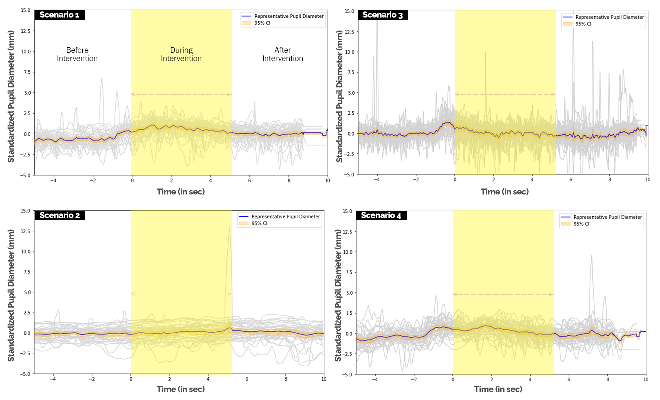
\includegraphics[width=0.95\linewidth]{images/fig1.pdf}
      \caption{Pupil dilation levels across scenarios and intervention types.}
      \label{fig:jaja}
    \end{figure}
 Median pupil diameters per driver \emph{j}, intervention phase and measurement occasion \texttt{timeindex} \emph{i} were extracted.
 
  \end{block}

  \begin{block}{Q2. Significance of interventions and criticality}
    To construct a multi-level model for addressing Q3, the \textit{Level 3} elements can be removed for a much simpler model, as there is:
    \begin{itemize}
        \item Neither significance between $T_1$ or $T_2$ intervention (\emph{p} = 0.932)
        \item Nor scenario critical situations, as also seen in Fig \textbf{\ref{fig:jaja}} (\emph{p} = 0.874)
    \end{itemize}

\begin{center}
    \textbf{\textcolor{utred}{Two-level linear mixed-effects model (LMEM) per driver \texttt{vp}:}}
\end{center}

\vspace{-0.4cm} % -ve space --

\begin{tcolorbox}[colback=gray!10, colframe=gray!50, sharp corners, boxrule=0.5pt, left=3pt, right=3pt, top=1pt, bottom=3pt, arc=0mm]
    \begin{align}
        \text{pdelt}_{ij} &= \beta_{0} + \beta_{1} \cdot \text{timeindex}_{ij} + \beta_{2} \cdot \text{age}_{ij} \nonumber \\
        &\quad + \beta_{3} \cdot \text{autexp}_{ij} + \beta_{4} \cdot \text{valence}_{ij} + b_{0j} + \epsilon_{ij}
    \end{align}
\end{tcolorbox}

\vspace{2cm}
\end{block}
\end{column}

\separatorcolumn

\begin{column}{\colwidth}

\begin{block}{Q3. LMEM Results}
\begin{table}
  \centering
  \begin{minipage}{0.45\textwidth}  % Adjust width as needed
    \centering
    \begin{tabular}{l r}
      \toprule
      \textt{Predictor} & \textt{\textit{p}-val} \\
      \midrule
      \texttt{age} & 0.058 \\
      \texttt{autexp} & 0.07 \\
      \bottomrule
    \end{tabular}
    \caption{Fixed effects}
    \label{susu}
  \end{minipage}%
  \hspace{0.05\textwidth} % Horizontal space between the tables
  \begin{minipage}{0.45\textwidth}  % Adjust width as needed
    \centering
    \begin{tabular}{l r}
      \toprule
      \textt{Group} & \textt{Variance} \\
      \midrule
      \texttt{vp} ($\beta_0$) & 3.61 \times 10^{-4} \\
      \textt{Residual}       & 2.42 \times 10^{-4} \\
      \bottomrule
    \end{tabular}
    \label{yaya}
    \caption{Random effects}
  \end{minipage}
\end{table}

Table \textbf{1} shows that older drivers have lesser dilation. Most drivers show similar baseline arousal levels. From Table \textbf{2}, a measure of inter-individual difference, is calculated as the ratio of \texttt{vp} variance to total (\texttt{vp} + residual) variance. The value is \emph{ICC} = \textbf{0.604} (high). 

\begin{table}
  \centering
  \begin{tabular}{l r r r r}
    \toprule
    \textt{\(\beta_{1} \text{ to } \beta_{4}\)} & \texttt{timeindex} & \texttt{age} & \texttt{autexp} & \texttt{valence} \\
    \midrule
    \texttt{timeindex} & -0.102 &      &       &       \\
    \texttt{age}       &  \textbf{-0.870} & 0.006 &       &       \\
    \texttt{autexp}    & \textbf{-0.398} & -0.002 & 0.121 &       \\
    \texttt{valence}   &\textbf{ -0.205} & -0.138 & -0.041 & 0.017 \\
    \bottomrule
  \end{tabular}
  \caption{Correlation between each predictor pair in the fixed effects.}
  \label{gugu}
\end{table}

From Table \textbf{\ref{gugu}}, drivers with prior automation experience have slightly lower arousal levels. Every additional exposure didn't result in drivers' pupil diameters \textit{adapting} to the experiment conditions. 

\end{block}

\begin{exampleblock}{Conclusion}
\begin{itemize}
    \item Neither authoritative control interventions ($T_1$ and $T_2$) nor scenario criticality significantly affect pupil dilation.
    \item Older participants and those with prior automation experience showed slightly lower pupil dilation, indicating potential familiarity with automation.
    \item Limited statistical power prevents firm conclusions.
    \item A wide age range and diverse participant backgrounds may have contributed to significant individual variations.
    \item Driver control inputs (ex. steering angle), offer much better arousal insights. Although while measuring physiological signals like pupil diameter, it is important to hence measure additional genetic and psychological measures that impact pupil dilation.
    \item Known approaches like data triangulation would help us better interpret arousal in such settings.
    
\end{itemize}
    
\end{exampleblock}
\end{column}

\separatorcolumn
\end{columns}
\end{frame}

\end{document}
